\documentclass{article}

\usepackage[margin=1in]{geometry}
\usepackage{tikz}
\usetikzlibrary{arrows.meta, positioning}
\begin{document}

\begin{figure}[h]
\centering

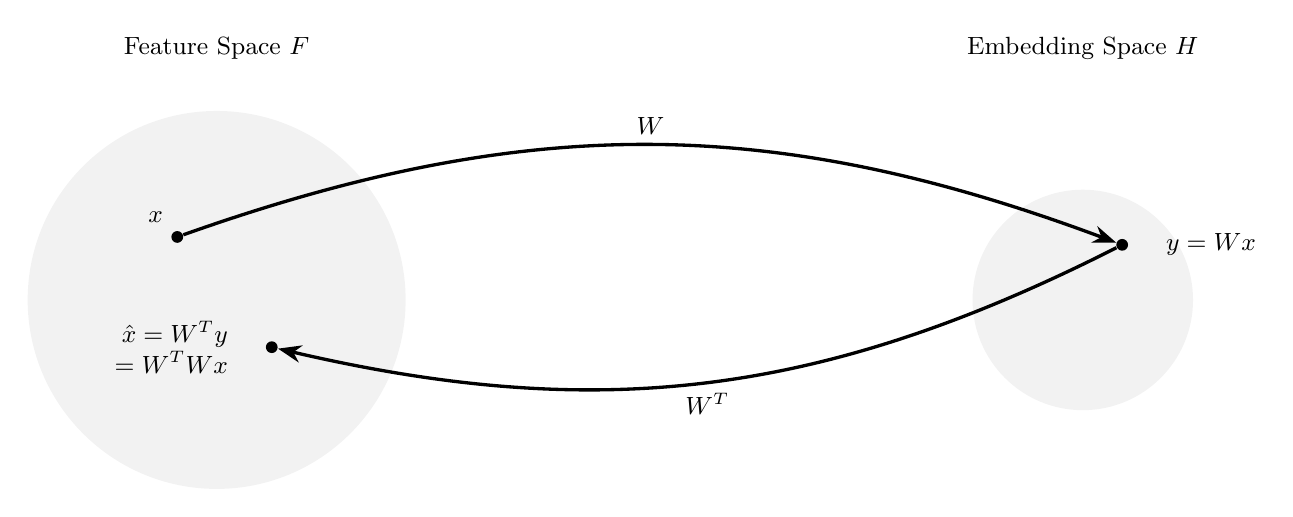
\begin{tikzpicture}[
    >=Stealth,
    font=\small,
    map/.style={->, very thick},
    point/.style={circle, fill, inner sep=1.5pt}
]

% --- Background spaces (light gray, no border) ---
\fill[gray!10] (-2.5,-2) circle (2.4);
\fill[gray!10] (8.5,-2) circle (1.4);

% Labels for spaces
\node at (-2.5,1.2) {Feature Space \(F\)};
\node at (8.5,1.2) {Embedding Space \(H\)};

% --- Points in F ---
\node[point, label=above left:\(x\)] (x) at (-3.0,-1.2) {};

\node[point] (xhat) at (-1.8,-2.6) {};
\node[left=10pt of xhat, align=right] {
\(\hat{x} = W^T y\) \\
\(\;\;= W^T W x\)
};

% --- Point in H ---
\node[point] (y) at (9.0,-1.3) {};
\node[right=10pt of y] {\(y = Wx\)};

% --- Arrows ---
\draw[map] (x) to[bend left=20]
    node[midway, above] {\(W\)}
    (y);

\draw[map] (y) to[bend left=20]
    node[midway, below] {\(W^T\)}
    (xhat);

\end{tikzpicture}

\caption{Feature embedding and recovery.}
\end{figure}

\end{document}